\section{Transition curves inherited from Paper 2}\label{sec:curves}

We use the following results of Paper~2 \citep{Paper2} as \emph{frozen inputs}: they are quoted, not re-proved, and
Paper~2 is used read-only (its archive is authenticated by SHA-256 in the repository, \cref{sec:repro}). Lemma names
are those of the Paper~2 manuscript; \cref{app:correspondence} gives the correspondence with the repository labels. With
$X=2^{-r/2}$, $Y=3^{-r/2}$, $W_r=1+X+Y/3$:
\begin{itemize}[leftmargin=1.5em]
\item \textbf{$\Atwou$ block} (Paper~2, Lemma~A). In the unit-edge normalisation the $\Atwou$ eigenvalue is
$\lambda_{\Atwou}=qW_q\,[h_A(p)-h_A(q)]$ with
\begin{equation}\label{eq:hA}
h_A(r)=\frac{2(r+1)X-4}{W_r}.
\end{equation}
$h_A$ increases on $(0,\rstar)$ and decreases strictly on $(\rstar,\infty)$, with $\rstar=1.4749107381\ldots$. For
$0<q<\rstar$ there is a unique $P_A(q)>\rstar$ with $h_A(P_A(q))=h_A(q)$; $\lambda_{\Atwou}>0$ for $q<p<P_A(q)$ and
$\lambda_{\Atwou}<0$ for $p>P_A(q)$. $P_A(0^+)=3.1054933552\ldots$.
\item \textbf{$\Ttwog$ block} (Paper~2, Lemmas~T0--T3). $K=qW_q\,[M(p)-M(q)]$ with
\begin{equation}\label{eq:M}
M(r)=\frac{1}{W_r}\begin{pmatrix} rX+\frac{2(2r+1)}{9}Y-2 & \frac{2\sqrt2(r+2)}{9}Y\\[2pt]
\frac{2\sqrt2(r+2)}{9}Y & 2r+\frac{2(r-1)}{9}Y-2\end{pmatrix}.
\end{equation}
$\tr K>0$ for all $p>q>0$ (Lemma~T1). With $D(p,q)=\det[M(p)-M(q)]$: for $0\le q<\qc$ there is exactly one
$p=P_T(q)>q$ with $D(p,q)=0$, and $\partial_pD(P_T(q),q)<0$ (Lemma~T3); the constant $\qc=2.0199382317\ldots$ is the
unique sign change of $\det M'$ (Lemma~T2), and $P_T(0^+)=4.7963681893\ldots$.
\item \textbf{Stable and unstable blocks} (Lemmas~S, E, T4). $\Aonegg$, $\Eg$, the internal $\Toneu$ and $\Ttwou$ are
positive for all $p>q>0$; $\Eu$ is negative for all $p>q>0$; $D\le0$ implies $h_A(p)<h_A(q)$, so on the $\Ttwog$
curve the $\Atwou$ eigenvalue is negative.
\item \textbf{Morse index of the cube} (Paper~2, Theorem~2). The index is
$2+\one\{q\ge\rstar\text{ or }p>P_A(q)\}+3\cdot\one\{q\ge\qc\text{ or }p>P_T(q)\}$ and the nullity (beyond the rigid
motions) is $\one\{q<\rstar,\,p=P_A(q)\}+3\cdot\one\{q<\qc,\,p=P_T(q)\}$; the two curves have no common point.
\item \textbf{Scale elimination} (Paper~2, Proposition~2.1). Minimising over scale, $V_*=-K\,\Phi_{p,q}^{1/(p-q)}$
with $\Phi_{p,q}=U_q^{\,p}/U_p^{\,q}$ and a positive constant $K$.
\end{itemize}

\begin{figure}[t]
\centering
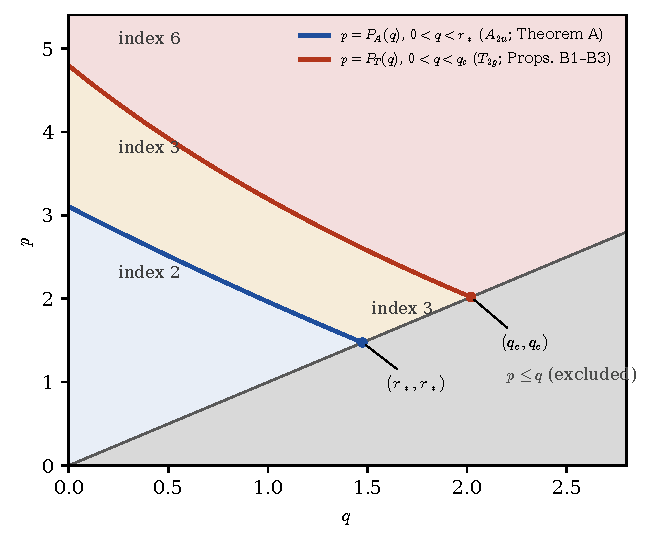
\includegraphics[width=0.62\textwidth]{figures/fig1_parameter_plane.pdf}
\caption{The parameter plane. The two transition curves of Paper~2, $p=P_A(q)$ for $0<q<\rstar$ and $p=P_T(q)$ for
$0<q<\qc$, end on the diagonal at $(\rstar,\rstar)$ and $(\qc,\qc)$ and never meet. The curves are drawn from their exact
definitions, evaluated at 30 significant digits by the project's root finders; their properties are proved in
Paper~2. The shading and the index labels illustrate Paper~2's index formula for the cube and are not a result of
this paper. The local branch results of this paper hold near each point of the two open curves.}
\label{fig:plane}
\end{figure}

\paragraph{Block signs on the $\Ttwog$ curve.} \Cref{tab:blocks} lists the signs that Paper~2's Theorem~2(b)--(d)
gives on $p=P_T(q)$, $0<q<\qc$. They are used only in \corBthree.

\begin{table}[h]
\centering\small
\caption{Hessian blocks of the cube on the physical $\Ttwog$ curve (frozen inputs from Paper~2).}\label{tab:blocks}
\begin{tabular}{lccl}
\toprule
block & dim & sign & source (Paper~2)\\
\midrule
$\Aonegg$ & 1 & $+$ & Lemma S\\
$\Eg$ & 2 & $+$ & Lemma S\\
$\Tonegg$ (rotations) & 3 & $0$, rigid, excluded & setup\\
$\Ttwog$ lower (critical) & 3 & $0$, the centre space $E_c$ & Lemmas T1, T3\\
$\Ttwog$ upper (noncritical copy) & 3 & $+$ & Lemma T1\\
$\Atwou$ & 1 & $-$ & Lemma T4\\
$\Eu$ & 2 & $-$ & Lemma E\\
$\Toneu$ (translations) & 3 & $0$, rigid, excluded & setup\\
$\Toneu$ (internal) & 3 & $+$ & Lemma S\\
$\Ttwou$ & 3 & $+$ & Lemma S\\
\bottomrule
\end{tabular}
\end{table}
